

This is example code from excercise 1: 

\begin{lstlisting}
# time plot of U.S. GNP and various fitted trends
par(mfrow=c(2,2))
par(oma=c(0,2,4,2))

# global quadratic trend
plot(x=1947.25+gnp.t,y=gnp.v,type="b",ylim=c(200,800),xlab="time",ylab="U.S. GNP",main="Global quadratic trend",col="green4")
lines(1947.25+gnp.t,predict(object=gqt.lm),col="blue")
legend(x="topleft",legend=c("actual values","estimated global trend"),col=c("green4","blue","red"),lty=c(1,1),pch=c(1,-1))

# global cubic trend
plot(x=1947.25+gnp.t,y=gnp.v,type="b",ylim=c(200,800),xlab="time",ylab="U.S. GNP",main="Global cubic trend",col="green4")
lines(1947.25+gnp.t,predict(object=gct.lm),col="blue")

# global multiplicative exponential trend
plot(x=1947.25+gnp.t,y=gnp.v,type="b",ylim=c(200,800),xlab="time",ylab="U.S. GNP",main="Global multiplicative exponential trend",col="green4")
lines(1947.25+gnp.t,exp(predict(object=gmet.lm)),col="blue")

# global additive exponential trend
plot(x=1947.25+gnp.t,y=gnp.v,type="b",ylim=c(200,800),xlab="time",ylab="U.S. GNP",main="Global additive exponential trend",col="green4")
lines(1947.25+gnp.t,predict(object=gaet.nls),col="blue")

mtext(text="Time plots of U.S. GNP and fitted trends",side=3,line=0,outer=T)
\end{lstlisting}

\begin{figure}[ht]
\centering
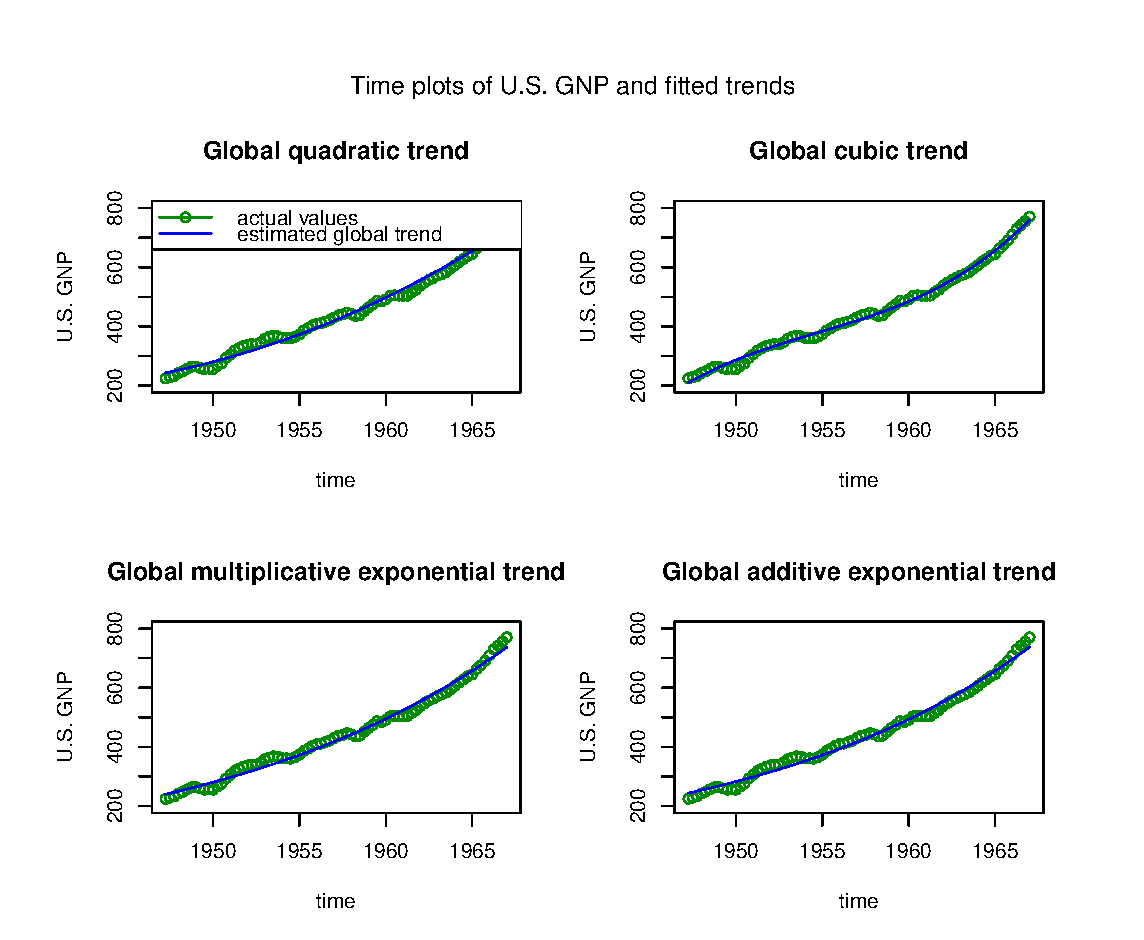
\includegraphics[width=0.8\textwidth]{plots/Rplot1.pdf}
\caption{various fits}
\end{figure}